% Computer Architecture (4190.308) Fall 2016 
% Seoul National University CARES Lab
% Lab 3 documentation

% Lines that need modification : 25~27

\documentclass{article}
\usepackage{graphicx, caption, subcaption, verbatim, moreverb, alltt, kotex}
\usepackage[protrusion=true,expansion=true]{microtype}
\usepackage{fancyvrb}
\let\verbatiminput=\verbatimtabinput

\setlength{\oddsidemargin}{0.25in}	% 1.25in left margin 
\setlength{\evensidemargin}{0.25in}	% 1.25in left margin (even pages)
\setlength{\topmargin}{0.0in}		% 1in top margin
\setlength{\textwidth}{6.0in}		% 6.0in text - 1.25in rt margin
\setlength{\textheight}{9in}		% Body ht for 1in margins
\addtolength{\topmargin}{-\headheight}	% No header, so compensate
\addtolength{\topmargin}{-\headsep}	% for header height and separation

% type user-defined commands here

\begin{document}

\title{Lab 3: Linear Pipelined and Circular Multi-cycle FFT Implementation}   % type title between braces
\author{CSE 4190.308 Computer Architecture \\ 3 Exercises (Total 100 Points)}         
\date{Received: March 26, 2016 \\Due: 11:00 a.m., April 4, 2016\\ \ \\TA Office Hours: 7:00 - 8:00 p.m., 4/1, 4/2, 4/3}    % type date between braces
\maketitle

\section{Introduction}
You will build up different versions of the FFT module which was discussed in
class, starting with a combinational FFT module (Figure 1). At first, you should examine
how the predefined combinational FFT is implemented by reading the source code.
Then, you have to implement a folded 3-stage multi-cycle FFT module, a pipelined 
3-stage FFT module and a super-folded version using multiple butterfly units. 
You can get more information in the lecture notes (\textit{Folding Complex Combinational 
Circuits to Save Area} and \textit{Pipelining Combinational Circuits}).
All code changes for this lab will be restricted to the file \emph{src/Fft.bsv}.

\begin{figure}[!h]
\centering
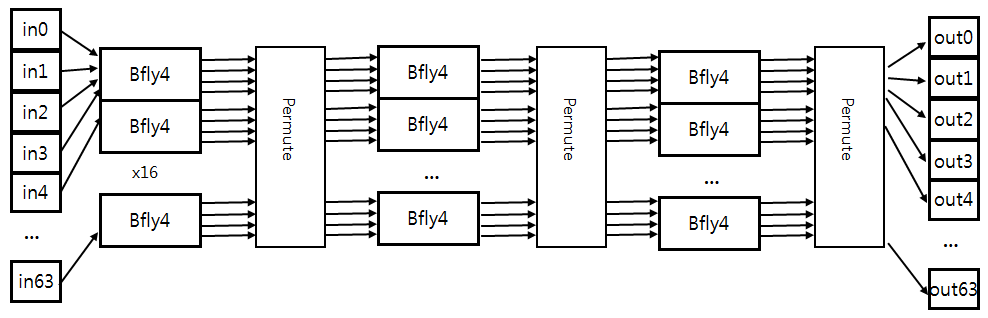
\includegraphics[width=0.8\textwidth]{figs/comb.png}
\caption{Combinational FFT}
\label{Comb}
\end{figure}

\section{Getting Started}
% (If you need a language assistance, please see our English-speaking TAs.)
\subsection{How to Download the Source Code}
% As we memtioned before, every assignments on this course will be managed in our svn server.
% You can get the skeleton source codes of Lab 2 by executing the script file \texttt{add-lab2.sh}
% which can be found on the course web page. Put the script in upper directory of your assignment directory named as your ID.
컴퓨터 구조 과목에서 사용하게 될 모든 실습은 이전에도 언급되었듯이 svn 서버를 통해 관리됩니다.
Lab 3의 실습 코드를 받는 방법은 역시 기존 lab들과 동일합니다.
수업 홈페이지에 올라와 있는 \texttt{add-lab3.sh} 스크립트를 다운받고,
기존 lab들을 수행했던 실습 디렉터리의 상위에 위치시킵니다.

\begin{Verbatim}[frame=single]
	$ ls
	add-lab3.sh YOUR_ID
	$ ls ./YOUR_ID/
	lab0 lab1 lab2 lab3
\end{Verbatim}
% The script file receives an ID as its first argument.
% You should give your own ID you've created before using the \texttt{student-create.sh} script.
% A password of archi13 can be required while you executing the script.
% It is the same password with the one of our course web page.
그 후 아래 예제와 같이 본인의 ID를 인자로 스크립트를 실행하셔야 합니다.
이 아이디는 여러분이 첫 실습 과제에 앞서 \texttt{student-create.sh} 스크립트로 생성한 아이디입니다.
코드를 다운 받는 과정에서 archi14의 password를 요구할 경우 강의 홈페이지와 동일한 비밀번호를 입력하시면 됩니다.

\begin{Verbatim}[frame=single]
	$ ./add-lab3.sh YOUR_ID
	Getting source codes for YOUR_ID
	archi16@hyewon.snu.ac.kr's password: 
\end{Verbatim}
% You can see a few messages like following after the source codes are downloaded completely.
아래와 같은 메세지가 보이면 실습 코드 다운이 완료된 것입니다.
\begin{Verbatim}[frame=single]
	Transmitting file data .....
	Committed revision 22.
	$
\end{Verbatim}

\subsection{Directory Structure of Lab 3}
% This is a brief description on directories and files which composes Lab 2.
Lab 3 실습의 디렉터리 구조는 다음과 같습니다.

\begin{figure*}[!h]
\begin{verbatim}
    lab3/	
        build/
        lib/
            TestBench.bsv
            ...
        src/
            Fft.bsv
            Makefile
            test
\end{verbatim}
\caption{Directory structure of Lab 3}
\label{fig:files}
\end{figure*}

\begin{description}
\item [\texttt{build}]\hfill \ \\
% Files generated while compling source codes will be located here.
컴파일 시 생성되는 파일들 및 메타 데이터들이 위치하는 폴더입니다.

\item [\texttt{lib}]\hfill \ \\
	% 
	실습에 사용되는 library 파일들이 위치하는 폴더입니다.
	실습을 하면서 수정할 필요 없는 파일들을 포함하고 있습니다.

\item [\texttt{src}]\hfill \ \\ 
	%
	실습에서 수정해야 할 파일들이 위치하는 폴더입니다.
	아래 지시사항에 따라 이 폴더에 있는 파일의 구현을 완성해야 합니다.

\item [\texttt{src/Fft.bsv}]\hfill \ \\
	%
	FFT 알고리즘을 수행하는 모듈이 구현될 파일입니다.
	사전에 구현된 combinational한 기존 FFT 모듈을 기반으로 하여
	세 가지 서로 다른 구현을 완성해야 합니다.
	구현해야 하는 모듈들은 뼈대코드의 형태로 주어집니다.

\item [\texttt{src/Makefile}]\hfill \ \\
	%
	Lab 3 코드의 컴파일 관련 명령 및 세부적인 사항이 정의되어 있습니다. \texttt{make} 명령을 통해
	Bluespec 코드의 컴파일이 가능하게 해줍니다.

\item [\texttt{src/test}]\hfill \ \\
	%
	이 파일을 이용하여 컴파일이 완료된 후 lab 3을 실행시켜 볼 수 있습니다.

\end{description}

\subsection{How to Test the Design}
실습에서 제공되는 test-bench는 여러분이 구현할 세 가지 FFT 모듈의 동작을 확인합니다.
먼저 모듈의 컴파일은 

\begin{Verbatim}[frame=single]
    $ ./make [fold|pipe|sfol]
\end{Verbatim}
와 같은 명령을 통해 수행할 수 있습니다. \texttt{make} 명령만 수행할 경우 세 모듈을 모두 컴파일 하며,
인자로 모듈을 지정해 줌으로써 각각의 모듈을 컴파일할 수 있습니다.
컴파일이 정상적으로 완료되면 다음 명령으로 여러분이 구현한 모듈의 동작을 확인할 수 있습니다.

\begin{Verbatim}[frame=single]
    $ ./test {fold|pipe|sfol}
    PASSED
\end{Verbatim}
예시와 같이 \texttt{PASSED} 라는 메시지가 보이면 알고리즘이 정상적으로 동작하는 것입니다.

\subsection{How to Submit Your Design}
Lab 3 실습 코드의 최상위 디렉터리인  \texttt{lab3} 디렉터리에서
다음과 같이 \texttt{svn commit} 명령을 수행하면 수정된 파일들이 제출됩니다.
마지막에 다음과 같은 메시지가 나타나면 숙제 제출이 정상적으로 완료된 것입니다.

\begin{Verbatim}[frame=single]
    $ svn commit
    ...
    Sending         lab3/src/Fft.bsv
    Transmitting file data ...
    Committed revision 15.
\end{Verbatim}

\section{Data Types}
Multiple data types are provided to help with the implementation.  The default
settings for the provided types describe an FFT implementation that works with
64 of 64-bit complex numbers.  The type for the 64-bit complex data is defined
as \texttt{ComplexData}.  The FFT works with the bluespec \texttt{Complex} type
that is slightly different from what was discussed in class. It is provided
with all of the required arithmetic overloads.  \texttt{FftPoints} defines the
number of complex numbers, \texttt{FftIdx} defines the datatype required for
accessing a point in the vector, \texttt{NumStages} defines the number of
stages, \texttt{StageIdx} defines a datatype to access a particular stage and
\texttt{BflysPerStage} defines the number of butterfly units in each stage.
These type parameters are provided for your convenience, feel free to use any
of these in your implementations.

It should be noted that the goal of this lab is not to understand the FFT algorithm,
but rather to experiment with different control logics in a real-world application.
The \texttt{getTwiddle} and \texttt{permute} functions are provided with the
testbench for your convenience. However, their implementations are not strictly
adhering to the FFT algorithm, and may even change later.
It would be beneficial to focus not on the algorithm, but on changing the
control logic of a given datapath in order to inhance its characteristics.

\section{Butterfly unit}
The module \texttt{mkBfly4} implements a 4-way butterfly function which was
discussed in the lecture.
This module is instantiated exactly as many times as you use it in your code.
One of the goals of this lab is to experiment with folding multiple usages
of the butterfly unit into a single instance, and saving chip space
by having a fewer number of shared units.

\begin{verbatim}
interface Bfly4;
  method Vector#(4,ComplexData) bfly4
    (Vector#(4, ComplexData) t, Vector#(4, ComplexData) x);
endinterface

module mkBfly4(Bfly4);
  method Vector#(4,ComplexData) bfly4
    (Vector#(4, ComplexData) t, Vector#(4, ComplexData) x);
    ...
  endmethod
endmodule
\end{verbatim}

\begin{figure}[!h]
\centering
\vspace{-13pt}
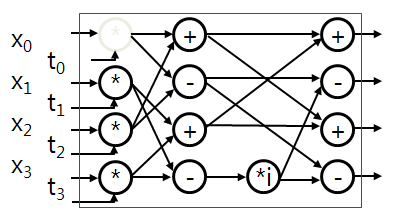
\includegraphics[width=0.4\textwidth]{figs/bfly.png}
\caption{Butterfly Unit}
\vspace{-13pt}
\label{bfly}
\end{figure}

\section{Different Implementations of the FFT}
You will be implementing modules corresponding to the following FFT interface:

\begin{verbatim}
interface Fft;
  method Action enq(Vector#(FftPoints, ComplexData) in);
  method ActionValue#(Vector#(FftPoints, ComplexData)) deq();
endinterface
\end{verbatim}

The modules \texttt{mkFftCombinational}, \texttt{mkFftFolded}, \texttt{mkFftPipelined}
and \texttt{mkFftSuperFolded} should implement all the 64-way FFT which is functionally equivalent
to the combinational model. 
The module \texttt{mkFftCombinational} is given to you.
Your job is to implement the other 3 modules, and demonstrate their correctness
using the provided combinational implementation as a benchmark.

Each of them contain two FIFOs \texttt{inFifo} and \texttt{outFifo} which contain the input
complex vector and the output complex vector respectively, as shown below.

\begin{verbatim} 
module mkFftCombinational(Fft);
  Fifo#(2,Vector#(FftPoints, ComplexData)) inFifo <- mkCFFifo;
  Fifo#(2,Vector#(FftPoints, ComplexData)) outFifo <- mkCFFifo;
\end{verbatim}

You will be learning about the FIFO modules in details sometime in the course.

Each module also contains a \texttt{Vector} or multiple \texttt{Vector}s of
mkBfly4, as shown below.

\begin{verbatim}
  Vector#(3, Vector#(16, Bfly4)) bfly <- replicateM(mkBfly4);
\end{verbatim}

The \texttt{doFft} rule performs the FFT algorithm and finally enqueues the
result into \texttt{outFifo}. This rule will usually require other functions
and modules to function correctly.

\begin{verbatim}
  rule doFft;
    ...
  endrule
\end{verbatim}

The \texttt{enq} method is used to send the input
vector to the FFT, while the \texttt{deq} method is used to dequeue the output
vector from the FFT.

\begin{verbatim}
  method Action enq(Vector#(FftPoints, ComplexData) in);
    inFifo.enq(in);
  endmethod

  method ActionValue#(Vector#(FftPoints, ComplexData)) deq;
    outFifo.deq;
    return outFifo.first;
  endmethod
endmodule 
\end{verbatim}

\noindent \paragraph{\bf Exercise 1 (25 pts):} 
In \texttt{mkFftFolded}, you should make use of just 16 butterflys overall, and
finish the overall FFT algorithm (starting from dequeuing the input FIFO to
enqueuing the output FIFO) in exactly 3 cycles.

\begin{figure}[!h]
\centering
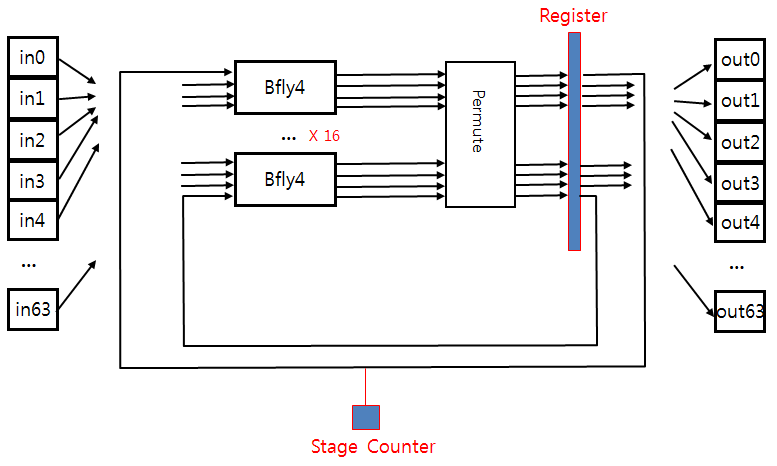
\includegraphics[width=0.8\textwidth]{figs/fold.png}
\caption{Folded FFT}
\label{fold}
\end{figure}

The makefile generates \texttt{simFold} that tests this implementation.
Compile and run using
\begin{verbatim}
$ make fold
$ ./test fold
\end{verbatim}

\noindent \paragraph{\bf Exercise 2 (30 pts):} 
In \texttt{mkFftPipelined}, you should make use of 48 butterflys overall, and
2 large registers, each carrying 64 complex numbers. 
The latency of this pipelined unit must also
be exactly 3 cycles, though it's throughput would be 1 FFT operation every
cycle.

\begin{figure}[!h]
\centering
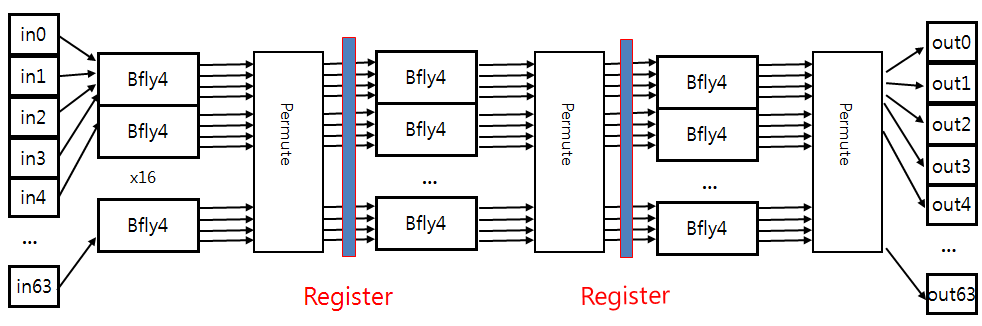
\includegraphics[width=0.8\textwidth]{figs/pipe.png}
\caption{Pipelined FFT}
\label{pipe}
\end{figure}

The makefile generates \texttt{simPipe} that tests this implementation.
Compile and run using
\begin{verbatim}
$ make pipe
$ ./test pipe
\end{verbatim}

\noindent \paragraph{\bf Exercise 3 (45 pts):} 
Finally, you will be implementing a polymorphic super-folded FFT module which
performs the FFT operation given a limited number of butterflys (either 1, 2,
4, 8, or 16). The parameter \texttt{radix} indicates the number of butterflys available
and the \texttt{times} means the necessary reused
number of each butterflys. Since \texttt{radix} 
is a type variable, we have to introduce it in the interface for the module. 
So we define a new interface called \texttt{SuperFoldedFft} as follows:

\begin{verbatim}
interface SuperFoldedFft#(radix);
  method Action enq(Vector#(64, ComplexData inVec));
  method ActionValue#(Vector#(64, ComplexData)) deq;
endinterface
\end{verbatim}

We also have to declare \textit{provisos} in the module
\texttt{mkFftSuperFolded} in order to inform the Bluespec compiler about the
arithmetic constraints among \texttt{radix}, \texttt{times} and \texttt{FftPoints} (namely that
\texttt{radix} and \texttt{times} are the factors for \texttt{FftPoints}/4. i.e. 
\texttt{radix} * \texttt{times} = \texttt{FftPoints}/4).

We finally instantiate a super-folded pipeline module with 4 butterflies, which
implements a normal \texttt{Fft} interface. This module will be used for
testing. We also show you the function which converts from a
\texttt{SuperFoldedFft\#(radix, n)} interface to an \texttt{Fft} interface.

\begin{figure}[!h]
\centering
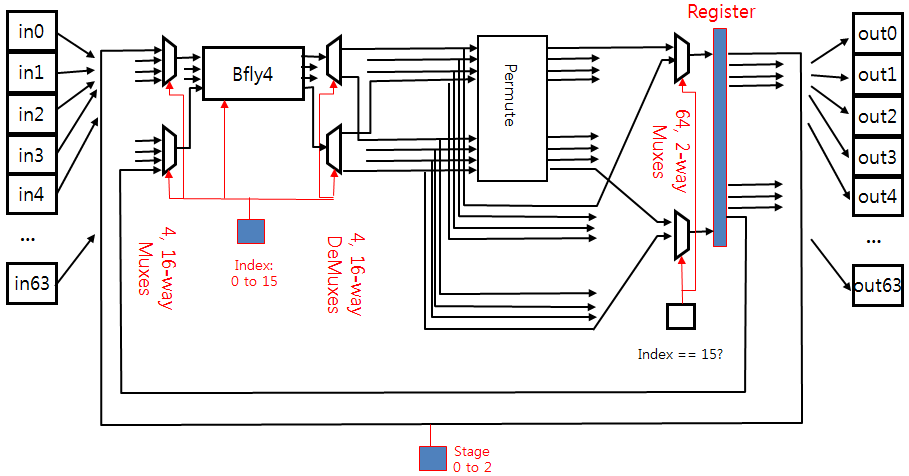
\includegraphics[width=0.8\textwidth]{figs/sfol.png}
\caption{Super Folded FFT (when \texttt{radix} = 1 and \texttt{times} = 16)}
\label{sfol}
\end{figure}

The makefile generates \texttt{simSfol} that tests this implementation.
Compile and run using
\begin{verbatim}
$ make sfol
$ ./test sfol
\end{verbatim}

The \texttt{Testbench} will automatically test the super-folded FFT module with 
all the possible radix values (i.e. 1, 2, 4, 8 and 16). 

In order to do the super-folded FFT module, first try writing a super-folded
FFT module with just 2 butterflys, without any type parameters. Then try to
extrapolate the design to use any number of butterflys.

\end{document}
